\scanpage{28}
\mspage{\handwritten{\unsure{2|7}2}}
% archive sheet number: 27 (inverted at the upper right)
% Source image 1683 x 2140. The whole-sheet cancellation is drawn at the end,
% using anchors in the text; deletion wrappers also record its textual state.
\noindent\begin{tikzpicture}[remember picture,overlay]
\coordinate (p28r1top) at (0,0);
\end{tikzpicture}%
\deleted{un morphisme de topos $\mathrm{u}:\mathrm{E}\handwritten{\longrightarrow}\mathrm{E}'$, et ce dernier sera ``unique à isomorphisme unique près'' en termes de la donnée $\mathrm{u}^{\handwritten{*}}$ resp. $\begin{tikzpicture}[baseline=(p28openingus.base),x=1em,y=1ex]
\node[inner sep=0pt] (p28openingus) at (0,0) {$\mathrm{u}_{\handwritten{*}}$};
\node[inner sep=0pt] at (.61,1.25) {\unsure{\begin{tikzpicture}[x=1em,y=1ex]\draw[gray,line width=.25pt] (0,0)--(.015,.35);\end{tikzpicture}}};
\end{tikzpicture}$, en un sens assez clair, et qui sera d'ailleurs entièrement explicité plus bas \handwritten{(\deleted{\unsure{2|3}}3.2.1)}\unsure{.}}

\deleted{\deleted{2}\handwritten{3}.1.2. Si $\mathrm{u}:\mathrm{E}\handwritten{\longrightarrow}\mathrm{E}'$ est un morphisme de topos, il résulte des propriétés des foncteurs adjoints
\mbox{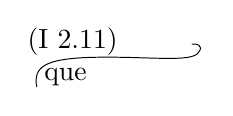
\begin{tikzpicture}[baseline=(p28r1que.base),x=1em,y=1em]
\node[anchor=base west,inner sep=0pt] (p28r1que) at (0,0) {que};
\node[anchor=base west,inner sep=0pt] at (-.6,1.15) {\inserted{\handwritten{(I 2.11)}}};
\draw[line width=.35pt] (-.25,-.25) .. controls (-.4,.5) and (.1,.75) .. (1.5,.82) .. controls (3.6,.9) and (5.4,.6) .. (5.6,1.02) .. controls (5.8,1.25) and (5.5,1.35) .. (5.35,1.3);
\end{tikzpicture}}
le foncteur image directe $\mathrm{u}_{\handwritten{*}}:\mathrm{E}\handwritten{\longrightarrow}\mathrm{E}'$ commute aux limites projectives, et le foncteur $\mathrm{u}^{\handwritten{*}}:\mathrm{E}'\handwritten{\longrightarrow}\mathrm{E}$ commute aux limites inductives}%
\margin{\handwritten{\deleted{(I \unsure{2.11|4.11})}.}}%
\deleted{ \deleted{\unsure{(2.11)|(I 2.11)}}\handwritten{\mbox{\begin{tikzpicture}[baseline=(p28r1star.base),x=1em,y=1em]
\node[inner sep=0pt] (p28r1star) at (0,0) {$(\phantom{*})$};
\node[inner sep=0pt] at (0,.55) {$*$};
% A definite star; two additional lower prongs have uncertain function.
\node[inner sep=0pt] at (.05,.12) {\unsure{\begin{tikzpicture}[x=1em,y=1em]
\draw[line width=.4pt] (-.12,.3) .. controls (-.2,.15) and (-.2,.04) .. (-.12,0);
\draw[line width=.4pt] (.03,.3) .. controls (.02,.16) and (.07,.06) .. (.08,0);
\end{tikzpicture}}};
\end{tikzpicture}}}.Comme on suppose de plus que ce dernier
\mbox{\begin{tikzpicture}[baseline=(p28r1commute.base),x=1em,y=1em]
\node[anchor=base west,inner sep=0pt] (p28r1commute) at (0,0) {commute};
\node[anchor=base west,inner sep=0pt] at (-3.4,1.2) {\inserted{\handwritten{est ex\unsure{.|a}ct à gauche i.e.}}};
\draw[line width=.35pt] (-.3,-.25) .. controls (-.6,.5) and (-.1,.8) .. (1.15,.9) .. controls (4.1,1.15) and (8.7,.95) .. (9.5,1.1) .. controls (9.9,1.16) and (10,1.35) .. (9.92,1.48);
% Detached point above the right end of the leader; function uncertain.
\node[inner sep=0pt] at (9.72,1.7) {\unsure{\begin{tikzpicture}\fill (0,0) circle (.35pt);\end{tikzpicture}}};
\end{tikzpicture}}
aux limites projectives finies, on voit donc en particulier que $\mathrm{u}^{\handwritten{*}}$ \uline{est} \deleted{exac} \uline{exact}.
\mbox{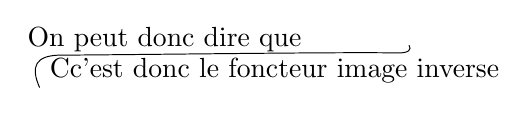
\begin{tikzpicture}[baseline=(p28r1cest.base),x=1em,y=1em]
\node[anchor=base west,inner sep=0pt] (p28r1cest) at (0,0) {\uline{\deleted{C}\handwritten{c}'est \deleted{donc} le foncteur image inverse}};
\node[anchor=base west,inner sep=0pt] at (-.8,1.12) {\inserted{On peut donc dire que}};
\draw[line width=.35pt] (-.35,-.35) .. controls (-.7,.45) and (-.45,.78) .. (.3,.82) .. controls (4.5,.85) and (10.9,.94) .. (12.6,.9) .. controls (13,.9) and (13.1,1.02) .. (13,1.18);
\end{tikzpicture}}
$\mathrm{u}^{\handwritten{\begin{tikzpicture}[x=.1cm,y=.1cm,baseline=0pt]
\draw[line width=.35pt] (0,.9)--(.6,-.6);
\draw[line width=.35pt] (.6,1)--(-.35,-.8);
\draw[line width=.35pt] (-.15,.1)--(1.3,.1);
\fill (.55,-1.0) circle (.11);
\end{tikzpicture}}}$ \deleted{qui}, dans le couple $(\mathrm{u}_{\handwritten{*}},\mathrm{u}^{\handwritten{\begin{tikzpicture}[x=.1cm,y=.1cm,baseline=0pt]
\draw[line width=.35pt] (-.20,1.0)--(.15,.05);
\draw[line width=.35pt] (-.5,0)--(1.1,0);
\draw[line width=.35pt] (.20,-.35)--(.40,-.88);
\fill (-.48,-.65) circle (.12);
\end{tikzpicture}}})$, \uline{qui possède les propriétés d'exactitude les plus remarquables}, \deleted{assurant} Ces propriétés assurent que pour toute espèce de structure algébrique
\mbox{\begin{tikzpicture}[baseline=(p28r1quipeut.base),x=1em,y=1em]
\node[anchor=base west,inner sep=0pt] (p28r1quipeut) at (0,0) {\deleted{qui}\texttt{x}\deleted{peut}};
% The x between the two cancelled words occupies their otherwise blank cell.
\node[anchor=base west,inner sep=0pt] at (0,1.15) {\inserted{\handwritten{$\Sigma$}}};
\draw[line width=.35pt] (-.25,-.35) .. controls (-.5,.3) and (-.1,.65) .. (1,.78) .. controls (2.5,.82) and (3.7,.93) .. (4,1.12) .. controls (4.15,1.22) and (4.1,1.4) .. (4.1,1.45);
% A separate faint short arc below Sigma, distinct from the insertion leader.
\node[inner sep=0pt] at (.45,.91) {\unsure{\begin{tikzpicture}[x=1em,y=1em]
\draw[line width=.2pt,gray] (0,.12) .. controls (.15,-.08) and (.48,-.04) .. (.72,.1);
\end{tikzpicture}}};
\end{tikzpicture}}
dont les données peuvent se décrire en termes de données de flèches entre les ensembles de base et des ensembles déduits de ceux-ci par \mbox{\begin{tikzpicture}[baseline=(p28application.base),x=1em,y=1ex]
\node[anchor=base west,inner sep=0pt] (p28application) at (0,0) {application};
% Two visible light diagonal stretches; ink versus surface origin is unresolved.
\node[inner sep=0pt,anchor=base west] at (0,0) {\unsure{\begin{tikzpicture}[overlay,x=1em,y=1ex]
\draw[gray,line width=.2pt] (-.15,3.1) -- (1.6,1.75);
\draw[gray,line width=.2pt] (4.0,-.10) -- (5.6,-2.25);
\end{tikzpicture}}};
\end{tikzpicture}} répétée d'opérations de limites projectives finies et de limites inductives quelconques,
\mbox{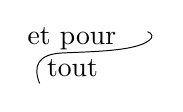
\begin{tikzpicture}[baseline=(p28r1tout.base),x=1em,y=1em]
\node[anchor=base west,inner sep=0pt] (p28r1tout) at (0,0) {tout};
\node[anchor=base west,inner sep=0pt] at (-.7,1.15) {\inserted{\handwritten{et pour}}};
\draw[line width=.35pt] (-.25,-.25) .. controls (-.5,.4) and (-.3,.8) .. (.55,.85) .. controls (1.5,.9) and (3.2,.9) .. (3.7,1.3) .. controls (3.9,1.42) and (3.8,1.58) .. (3.65,1.62);
\end{tikzpicture}}
\handwritten{``}objet de $\underline{\mathrm{E}}'$ muni d'une structure d'espèce $\handwritten{\Sigma}$'' (notion qui a un sens grâce aux propriétés d'exactitude \deleted{de} internes du topos
\mbox{\begin{tikzpicture}[baseline=(p28r1E.base),x=1em,y=1em]
\node[inner sep=0pt] (p28r1E) at (0,0) {$\mathrm{E}$};
% E is certain. The heavy lower material may be a second impression or pen work.
\node[inner sep=0pt] at (0,-.12) {\unsure{\begin{tikzpicture}[x=1em,y=1em]
\draw[line width=1.1pt] (-.28,0) -- (.3,0);
\draw[line width=.75pt] (.28,0) .. controls (.3,.13) and (.27,.24) .. (.2,.3);
\end{tikzpicture}}};
\node[inner sep=0pt] at (.49,.28) {$'$};
\end{tikzpicture}}
(II 4.1)), son image 
\begin{tikzpicture}[baseline=(p28inverse.base),x=1cm,y=1cm]
\node[anchor=base west,inner sep=0pt] (p28inverse) at (0,0) {\deleted{inverse}};
\draw[line width=.65pt] (-.08,.12)--(1.34,.12) .. controls (1.41,.12) and (1.46,.28) .. (1.50,.37);
\draw[line width=.55pt] (.02,-.12)--(.07,.38);
\end{tikzpicture} par $\mathrm{u}^{\handwritten{*}}$ est muni des mêmes structures. Plutôt que d'entrer dans la tâche peu engageante de donner un sens précis à cet énoncé et de le justifier de façon formelle, nous conseillons au lecteur de
\mbox{\begin{tikzpicture}[baseline=(p28r1se.base),x=1em,y=1em]
\node[anchor=base west,inner sep=0pt] (p28r1se) at (0,0) {se};
\node[anchor=base west,inner sep=0pt] at (-1.2,1.15) {\inserted{l'\begin{tikzpicture}[baseline=(p28expe.base),x=1em,y=1ex]
\node[inner sep=0pt] (p28expe) at (0,0) {e};
\node[inner sep=0pt] at (-.16,.61) {\unsure{\begin{tikzpicture}[x=1em,y=1ex]\draw[line width=.25pt] (0,.13)--(.21,-.15);\end{tikzpicture}}};
\end{tikzpicture}xpliciter et de}};
\draw[line width=.35pt] (-.25,-.28) .. controls (-.45,.4) and (-.15,.8) .. (.6,.86) -- (10.4,.86) .. controls (10.65,.86) and (10.7,1) .. (10.65,1.12);
\end{tikzpicture}}
convaincre de sa validité
\mbox{\begin{tikzpicture}[baseline=(p28r1pour.base),x=1em,y=1em]
\node[anchor=base west,inner sep=0pt] (p28r1pour) at (0,0) {pour};
% Three detached dark points below the gap following pour; no function assigned.
\node[inner sep=0pt] at (2.65,-.9) {\unsure{\begin{tikzpicture}[x=1em,y=1em]
\fill (.3,0) circle (.45pt);
\fill (.15,-.27) circle (.45pt);
\fill (0,-.56) circle (.35pt);
\end{tikzpicture}}};
\end{tikzpicture}}
des espèces de structure telles que celle de groupe, d'anneau, de module sur un anneau, de comodule \deleted{ou}\texttt{x}\deleted{de}\texttt{x}\deleted{bimodule} sur un anneau, de bigèbre sur un anneau, de torseur sous un groupe. (Dans ces exemples, les trois premières espèces de structure se définis}
% The two x impressions above occupy the two otherwise blank cells of the
% cancelled phrase. Final definis is cut at the right edge; the parenthesis stays open.
\noindent\begin{tikzpicture}[remember picture,overlay]
\coordinate (p28r1bodyend) at (0,0);
\end{tikzpicture}


\handwritten{\figure{
\begin{tikzpicture}[x=1cm,y=1cm]
\draw[line width=.4pt] (0,.03) .. controls (.8,-.08) and (1.0,-.05) .. (1.6,0) .. controls (4.8,.12) and (9.7,-.08) .. (13.0,.04) .. controls (13.5,.06) and (13.9,.10) .. (14.2,.03);
\end{tikzpicture}}}

\noindent\begin{tikzpicture}[remember picture,overlay]
\coordinate (p28r1footstart) at (0,0);
\end{tikzpicture}%
\deleted{($\handwritten{\begin{tikzpicture}[x=.1cm,y=.1cm,baseline=0pt]
\draw[line width=.35pt] (-.4,.7)--(.6,-.6);
\draw[line width=.35pt] (.2,1)--(-.2,-.1);
\draw[line width=.35pt] (-.6,.1)--(1,.1);
\fill (-.28,-.65) circle (.12);
\end{tikzpicture}}$) \deleted{On peut} \deleted{d}\handwritten{D}'ailleurs
\mbox{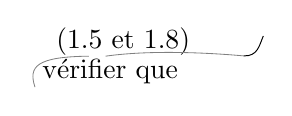
\begin{tikzpicture}[baseline=(p28r1verifier.base),x=1em,y=1em]
\node[anchor=base west,inner sep=0pt] (p28r1verifier) at (0,0) {\deleted{vérifier que}};
\node[anchor=base west,inner sep=0pt] at (.5,1.1) {\inserted{\handwritten{(1.5 et 1.8)}}};
% Three visible stretches: pale left return, interrupted middle, dark right upturn.
\draw[gray,line width=.3pt] (-.25,-.3) .. controls (-.5,.45) and (-.2,.8) .. (1.7,.82);
\draw[gray,line width=.3pt] (2.3,.82) .. controls (3.7,1.02) and (5.6,.98) .. (7.3,.83);
\draw[line width=.35pt] (7.3,.83) .. controls (7.8,.82) and (7.85,1.2) .. (8,1.55);
\end{tikzpicture}},pour un foncteur $\mathrm{u}_{\handwritten{\begin{tikzpicture}[x=.1cm,y=.1cm,baseline=0pt]
\draw[line width=.35pt] (-.30,.60)--(.20,.05);
\draw[line width=.35pt] (.50,.8)--(-.35,-.7);
\draw[line width=.35pt] (-.45,0)--(1,0);
\fill (.48,-.88) circle (.13);
\end{tikzpicture}}}:\mathrm{E}\handwritten{\longrightarrow}\mathrm{E}'$ resp. $\mathrm{u}^{\handwritten{\begin{tikzpicture}[x=.1cm,y=.1cm,baseline=0pt]
\draw[line width=.35pt] (-.30,.7)--(.25,.03);
\draw[line width=.35pt] (.15,1)--(-.15,-.6);
\draw[line width=.35pt] (-.2,.1)--(.9,.1);
\fill (.40,-.83) circle (.12);
\end{tikzpicture}}}:\mathrm{E}'\handwritten{\longrightarrow}\mathrm{E}$ donné, \deleted{d}\handwritten{c}e foncteur admet un adjoint à gauche (resp. à droite si et seulement si il commute aux
\mbox{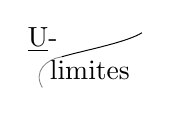
\begin{tikzpicture}[baseline=(p28r1limites.base),x=1em,y=1em]
\node[anchor=base west,inner sep=0pt] (p28r1limites) at (0,0) {limites};
\node[anchor=base west,inner sep=0pt] at (-.8,1.2) {\inserted{$\underline{\mathrm{U}}$-}};
\draw[gray,line width=.3pt] (-.25,-.28) .. controls (-.6,.3) and (-.1,.75) .. (.45,.83);
\draw[line width=.35pt] (.45,.83) .. controls (1.2,1.05) and (2.8,1.35) .. (3.35,1.7);
\end{tikzpicture}}
projectives (resp. aux $\underline{\mathrm{U}}$-limites inductives).
\mbox{\begin{tikzpicture}[baseline=(p28r1dailleurs.base),x=1em,y=1em]
\node[anchor=base west,inner sep=0pt] (p28r1dailleurs) at (0,0) {\deleted{\unsure{D'ailleurs}\unsure{,}}};
% An additional faint down-right tail below the cancelled word's end.
\node[inner sep=0pt] at (4.8,-.3) {\unsure{\begin{tikzpicture}[x=1em,y=1em]
\draw[line width=.25pt,gray] (0,0) .. controls (.2,-.1) and (.5,-.4) .. (.75,-.45);
\end{tikzpicture}}};
\end{tikzpicture}}
\deleted{c'est une conséquence immédiate de 1.2.\mbox{\begin{tikzpicture}[baseline=(p28subdiv.base),x=1cm,y=1cm]
\node[inner sep=0pt] (p28subdiv) at (0,0) {\unsure{(ii)|(iii)|(i)|(ii|(iii|(i}};
\node[inner sep=0pt] at (.535,.285) {\unsure{\begin{tikzpicture}[x=1cm,y=1cm]
\draw[gray,line width=.2pt] (-.135,.045) .. controls (-.045,-.005) and (.025,-.035) .. (.135,-.045);
\end{tikzpicture}}};
\draw[line width=.9pt] (.38,-.31) .. controls (.47,-.26) and (.61,-.29) .. (.72,-.27);
\end{tikzpicture}}}}
% The right image edge after droite contains no visible closing parenthesis.
\noindent\begin{tikzpicture}[remember picture,overlay]
\coordinate (p28r1footend) at (0,0);
\end{tikzpicture}
\handwritten{\figure{\begin{tikzpicture}[remember picture,overlay]
% Main long cancellation: one upper path, two detached points, one short
% segment near the raised footnote reference, and one continuing lower path.
\draw[line width=.35pt] ([xshift=.405\linewidth,yshift=-.65cm]p28r1top)
 .. controls ([xshift=.375\linewidth,yshift=-3cm]p28r1top) and ([xshift=.44\linewidth,yshift=4cm]p28r1bodyend)
 .. ([xshift=.38\linewidth,yshift=.35cm]p28r1footstart);
\fill ([xshift=.379\linewidth,yshift=.29cm]p28r1footstart) circle (.35pt);
\fill ([xshift=.378\linewidth,yshift=.23cm]p28r1footstart) circle (.35pt);
\draw[line width=.35pt] ([xshift=.377\linewidth,yshift=.18cm]p28r1footstart) -- ([xshift=.376\linewidth,yshift=.12cm]p28r1footstart);
\draw[line width=.35pt] ([xshift=.375\linewidth,yshift=.04cm]p28r1footstart)
 .. controls ([xshift=.36\linewidth,yshift=-.4cm]p28r1footstart) and ([xshift=.35\linewidth,yshift=.6cm]p28r1footend)
 .. ([xshift=.342\linewidth,yshift=.36cm]p28r1footend);
\node[inner sep=0pt] at (0,0) {\unsure{\begin{tikzpicture}[remember picture,overlay]
\draw[gray,line width=.3pt] ([xshift=.342\linewidth,yshift=.36cm]p28r1footend)
 .. controls ([xshift=.336\linewidth,yshift=.20cm]p28r1footend) and ([xshift=.33\linewidth,yshift=.04cm]p28r1footend)
 .. ([xshift=.325\linewidth,yshift=-.1cm]p28r1footend);
\end{tikzpicture}}};
\end{tikzpicture}}}

% The pale end of the long cancellation is retained as a lighter continuation.
% Small points and interrupted star rays are literal graphic details, not extra mathematical symbols.
% The diagonal near application has no assigned textual significance.
